\chapter*{Capitolo 2}
\addcontentsline{toc}{chapter}{Capitolo 2}

\section*{Tecnologie Utilizzate}
\addcontentsline{toc}{section}{Tecnologie Utilizzate}

\section*{Data-Plane Development Kit}
\addcontentsline{toc}{section}{Data-Plane Development Kit}

Data-Plane Development Kit è un framework sviluppato da Intel, con primo rilascio nel 2010 e ora supportato da The Linux Foundation. DPDK consiste in un set di librerie e di driver che consentono  di accelerare il packet processing.
Il suo punto di forza consiste nell'eseguire le applicazioni direttamente in user-space, in modo che vengano eseguite direttamente sulla NIC. 
Uno dei punti di forza di DPDK è la performance elevata su piccoli pacchetti di dati.
Un flusso di dati con pacchetti di piccole dimensioni (tipicamente 64 byte) viene gestito male dal Networking Stack di Linux perché genera un numero elevato di interrupt (uno per ogni pacchetto). Grazie ai Poll Mode Driver di cui fa uso DPDK, la gestione diventa a polling in modo da usare una minore quantità di interrupt.\\
DPDK sfrutta inoltre il Kernel Bypassig, così da non consultare il Networking Stack e avere prestazioni migliori.
Le applicazioni in questo modo riescono a dialogare direttamente con la NIC che riceve il traffico di dati, senza interferire con il Kernel.
DPDK è compatibile con un vasto numero di CPU, architetture e schede di rete. Gli obiettivi del set di librerie sono i seguenti.
\begin{itemize}
    \item Ricevere e inviare i pacchetti nel minor numero possibile di cicli della CPU, per massimizzare l'efficienza del Data Plane
    \item Catturare i pacchetti più velocemente possibile
    \item Essere compatibile con i Fast Path Stack di terze parti
\end{itemize} 
\pagebreak
In \textbf{Figura \ref{fig:helloworld_dpdk}} è presente l'esempio di un programma che stampa ``Hello World" con DPDK.
\FloatBarrier
\begin{figure}[h]
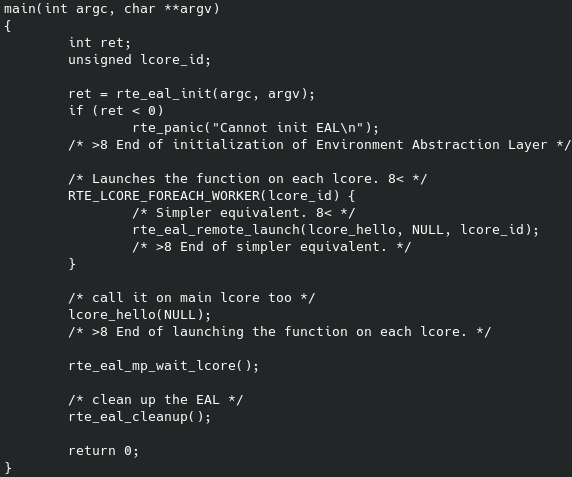
\includegraphics[width=7.5cm]{images/helloworld_dpdk.png}
\centering
\caption{\textit{Hello World con DPDK}}
\label{fig:helloworld_dpdk}
\end{figure}
\FloatBarrier
\section*{Kernel Bypassing}
\addcontentsline{toc}{section}{Kernel Bypassing}
DPDK adotta il Kernel Bypassing \cite{enberg_kernel-bypass_2018} e grazie a questo riesce a raggiungere prestazioni elevate.
Il Kernel Bypassing permette di saltare lo stack di networking che è presente nei sistemi operativi, ovvero i vari livelli che un pacchetto di rete deve percorrere per arrivare alla scheda di rete. La completa eliminazione del passaggio del pacchetto nello stack, è possibile grazie all' astrazione che DPDK introduce portando nello user-space le applicazioni. In questo modo il dialogo tra hardware e software non avviene più a livello del Kernel, ma viene portato sulla scheda di rete. Questo avvantaggia il processo di ricezione e invio del singolo dato perché soggetto ad una pipeline più breve e meno operazioni di copia. In \textbf{Figura \ref{fig:kernel_bypassing}} si mostra il livello di direttezza del Kernel Bypassing.

\FloatBarrier
\begin{figure}[h]
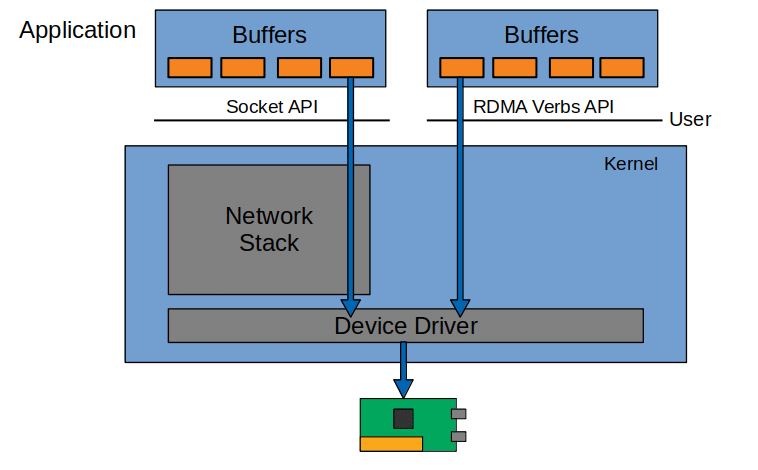
\includegraphics[width=8cm]{images/kernel_bypassing.png}
\centering
\caption{\textit{Accesso diretto alla NIC grazie al Kernel Bypassing}} \cite{noauthor_kernel-networking-vs-kernel-bypassingppm_nodate}
\label{fig:kernel_bypassing}
\end{figure}
\FloatBarrier

\subsection*{Vantaggi di DPDK}

\vspace{2mm}
\addcontentsline{toc}{subsection}{Polling}
\subsubsection*{Polling}
DPDK sfrutta i Poll Mode Drivers (PMD) ovvero una modalità a polling che si contrappone al classico modello ad interrupt e che è funzionale nel caso in cui si gestiscano enormi quantità di dati (esempio reti da \textbf{1 - 2 Gbit/s}).\\
Questa modalità prevede che assegnando, ad esempio, i core 1 e 2 (flag -l 0-1) su 4 core di sistema, i primi due core verranno dedicati interamente alla gestione del polling di DPDK. Questo succede perché vengono considerati in modalità non-preemptive e prioritaria: ogni volta che viene richiesto un pacchetto, i due core hanno la priorità di esecuzione sulla gestione di questo.
I pacchetti sono gestiti in code (queues) e la CPU li può leggere in base al carico  dati che ha in quel momento.\\
La CPU notifica la NIC nel momento in cui è possibile leggere altre code e così la NIC può inviare nuovamente l'interrupt per i prossimi dati.

\vspace{2mm}
\addcontentsline{toc}{subsection}{Zero Copy}
\subsubsection*{Zero Copy}
Nel corso dell' arrivo di un pacchetto e del successivo processamento, una nuova copia viene generata all'interno dell'applicazione che lo ha richiesto. Con DPDK, avendo la NIC il diretto accesso ai pacchetti, si dimezza il tempo necessario in quanto le librerie di cui fa uso consentono di impiegare direttamente i dati in arrivo, in modo ``raw" (la NIC ne prende totalmente carico), senza doverli copiare.

\vspace{2mm}
\addcontentsline{toc}{subsection}{User Defined Ring Buffer}
\subsubsection*{User Defined Ring Buffer}
DPDK delega completamente e in modo trasparente alla NIC la gestione del pacchetto e quindi il Kernel non attiva nessun ring.
\leavevmode\newline
In \textbf{Figura \ref{fig:dpdkdifferences}} sono presentate le differenze tra un sistema che usa DPDK e un sistema che non lo usa.
\FloatBarrier
\vspace{1cm}
\begin{figure}[h]
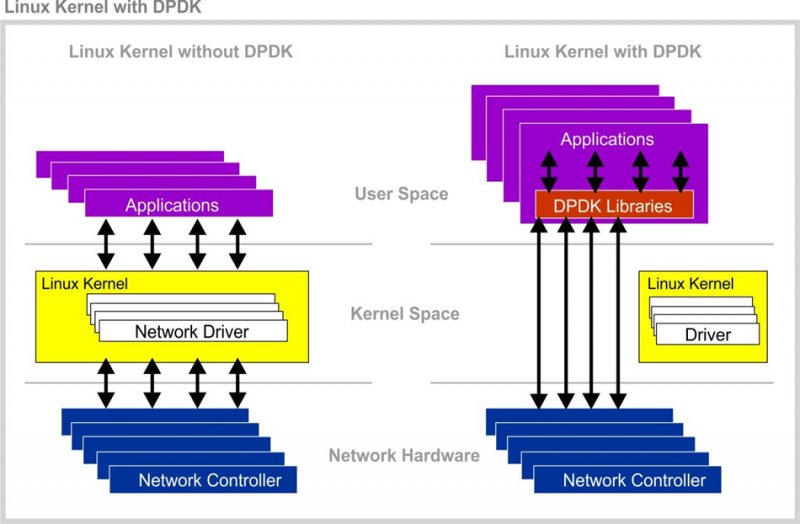
\includegraphics[scale=0.30]{images/dpdkdifferences.png}
\centering
\caption{\textit{Vantaggi di DPDK}}
\label{fig:dpdkdifferences}
\end{figure}
\FloatBarrier

\addcontentsline{toc}{section}{DPDK nel dettaglio}
\subsubsection*{DPDK nel dettaglio}
Il set di librerie che DPDK offre è diviso in molti punti chiave. Riassumendo, il ``core" del framework è suddiviso nei seguenti componenti.
\begin{itemize}
    \item \textbf{Memory Manager} responsabile dell' allocazione di pool di oggetti in memoria
    \item \textbf{Buffer Manager} prealloca la memoria necessaria pronta per l'uso all'esecuzione di DPDK
    \item \textbf{Queue Manager} implementa le code utilizzabili se supportate dalla scheda di rete, sia per la ricezione che per la trasmissione
    \item \textbf{Flow Classification} permette di introdurre i pacchetti più velocemente nel flusso di dati
    \item \textbf{Poll Mode Drivers} evita di usare il meccanismo classico ad interrupt. Dei core della CPU si dedicano completamente al polling rendendo la CPU sempre disponibile alla ricezione o all'invio di pacchetti.
\end{itemize}

\addcontentsline{toc}{subsection}{Hugepages}
\subsection*{Hugepages}
Le Hugepages sono blocchi di memoria di dimensione variabile, composti da singole pagine da 4096 byte. DPDK utilizza le ``Persistent Hugepages" allocate in modo dinamico, più stabili delle tipiche ``Transparent Hugepages" che sono allocate a runtime in modo automatico.\\
Usando pagine di grande dimensione è possibile accedere alla memoria più velocemente. Queste sono infatti preallocate per l'esecuzione del programma e permettono di migliorare le performance del sistema, non dovendo allocare memoria per ogni operazione richiesta. 
Secondo la documentazione di DPDK è consigliato usare Hugepages da 1GB, ovvero preallocare 256.000 pagine di memoria.\\
Conseguentemente al grande numero di pacchetti che si deve gestire, essendo DPDK pensato per gestire flusso dati su larga scala, si utilizzano le hugepages per evitare di accedere al disco per ogni pacchetto in arrivo. La memoria è preallocata e non ha bisogno di essere riallocata per ogni operazione di rete: si evitano molti problemi e si garantisce velocità di lettura.
Usando normali pagine si avrebbero molte più entry da controllare, ciò risulterebbe in un maggiore ``tempo di burst" per la CPU.\\
Le hugepages possono essere da 2M o da 1GB. Nel caso di una Virtual Machine si possono usare 2048K di pagine per far funzionare correttamente la suite DPDK. Per lo studio delle prestazioni in trasmissione e ricezione sono state usate delle pagine da 1GB all' interno di una macchina virtuale.

\addcontentsline{toc}{subsection}{Environment Abstraction Layer (EAL)}
\subsection*{Environment Abstraction Layer (EAL)}
L' Environment Abstraction Layer è il responsabile dell'accesso alle risorse a basso livello e alla memoria. È un livello generico di astrazione che permette di eseguire DPDK senza che esso conosca l'hardware sottostante. I compiti dell' EAL sono molteplici, come ad esempio avviare DPDK, assegnare le istruzioni agli specifici core e riservare zone di memoria per le interazioni con la scheda di rete.\\
Per il setup, il programma ha bisogno della funzione \textbf{rte\_eal\_init()} che inizializza l' Enviroment Abstraction Layer in modo da accedere alle risorse di basso livello. In particolare utilizzando le librerie \textbf{pthread} possiamo delegare ogni esecuzione ad un thread diverso (ad esempio in una macchina con 4 core che dispone di hyperthreading ad 8 thread, si può lanciare il programma delegando a tutti gli 8 core i vari processi).
L'inizializzazione come ogni programma \textbf{C} è delegata alla glibc, ma l'inizializzazione effettiva è una chiamata alle librerie phread eseguita tramite rte\_eal\_init().
Al termine del programma, per la deallocazione delle risorse si ha una chiamata a \textbf{rte\_eal\_cleanup()}
In \textbf{{Figura \ref{fig:EAL}}} è mostrata l'inizializzazione delle EAL al lancio del programma con la conseguente creazione dei pthread. È quindi intuibile da questo tipo di startup che il programma sia stato eseguito su due core e quindi utilizzando gli specifici parametri EAL \begin{minted}[escapeinside=||]{py}
./program |\colorbox{lightgray}{-l 2}|
\end{minted}
\FloatBarrier
\begin{figure}[h]
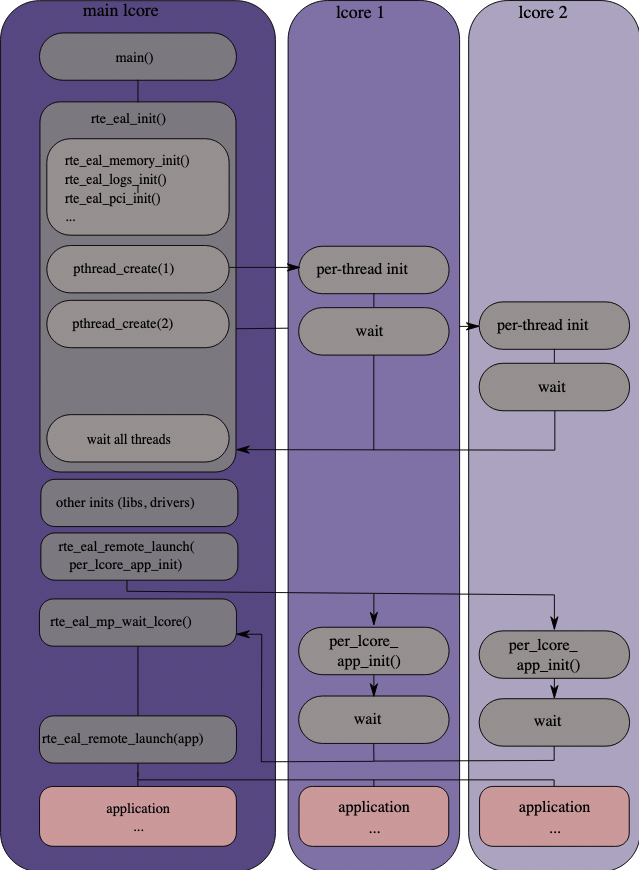
\includegraphics[scale=0.40]{images/EAL.png}
\centering
\caption{\textit{Inizializzazione dell' EAL}}
\label{fig:EAL}
\end{figure}
\FloatBarrier
\addcontentsline{toc}{subsection}{Poll Mode Drivers (PMD)}
\subsection*{Poll Mode Drivers (PMD)}
I Poll Mode Driver sono un set di API che hanno accesso ai canali di comunicazione in ricezione e trasmissione senza la necessità di utilizzare interrupt. Hanno la funzionalità di configurare i devices e le loro code e funzionano completamente nello user-space. Hanno il compito di processare e inviare i pacchetti nel modo più ottimizzato possibile e in base alle condizioni di carico del sistema al momento e sono configurabili ``on the fly".

\pagebreak
\addcontentsline{toc}{section}{Programming Protocol-Indipendent Packet Processors: P4}
\section*{Programming Protocol-Indipendent Packet Processors: P4}

P4 è un linguaggio di programmazione ad alto livello che abbraccia completamente il concetto di SDN, essendo ``Protocol Indipendent" \cite{noauthor_p4_nodate}. Permette allo sviluppatore di implementare uno Networking Stack personale in hardware di rete come switch o router. La forza di P4 è dare al programmatore tutti gli strumenti necessari per programmare dispositivi di switching in modo da essere facilmente configurabili sulla base di esigenze sempre nuove, come l'introduzione di nuovi header. Grazie alla sua versatiltà può essere introdotto in router, switch o altri dispositivi di rete che processano pacchetti. P4 può essere applicato e  compilato per un grande numero di dispositivi che vengono chiamati ``Targets". Per ogni dispositivo su cui agisce P4, possono essere predisposte diverse regole.

\addcontentsline{toc}{subsection}{Architettura}
\subsubsection*{Architettura}
L'architettura PSA (Portable Switch Architecture) \cite{noauthor_p4_2022} descrive le caratteristiche principali che hanno dispositivi di rete come switch, per processare ed inoltrare pacchetti. PSA contiene la libreria di tipi e costrutti disponibili per programmi P4 standard.
Il modello PSA ha sei ``Programmable Blocks" e due ``Fixed Function Blocks". I blocchi sono programmabili tramite P4, mentre i restanti due blocchi dipendono dal target sul quale sono applicati. In \textbf{{Figura \ref{fig:pipeline_p4}}}
 si vede la classica pipeline di una PSA.
\vspace{1cm}
\begin{figure}[h]
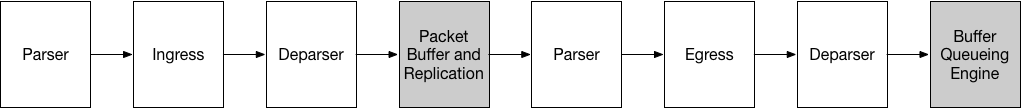
\includegraphics[scale=0.4]{images/pipeline_p4.png}
\centering
\caption{\textit{PSA Pipeline}}
\label{fig:pipeline_p4}
\end{figure}
\leavevmode\newline
Con questa pipeline si validano i pacchetti in arrivo al dispositivo di rete e si applicano le regole che sono stabilite su ingress (match + action). Il primo Function Block permette all'evenienza di duplicare i pacchetti per funzionalità future. Alla fine della pipeline il pacchetto viene serializzato e spedito dal secondo Function Block ai successivi riceventi.
\addcontentsline{toc}{subsection}{Header}
\subsubsection*{Header}
P4 può supportare una gamma di protocolli così vasta grazie alla riconfigurabilità che hanno i suoi header. Gli header di un pacchetto P4 infatti possono essere definiti in modo personalizzato così che si possano adattare all'esigenza della rete, in modo che all'aggiunta in rete di nuovi protocolli, il programma P4 si possa adattare ai nuovi pacchetti. La sintassi degli header è simile a quella delle strutture in C.

\addcontentsline{toc}{subsection}{Parser e Deparser}
\subsubsection*{Parser e Deparser}
Un programma P4 deve essere disposto di un parser e di un deparser \cite{noauthor_notitle_nodate}. Il parser serve a collegare la rappresentazione a bit del pacchetto alla reale struttura dati che lo rappresenta nel linguaggio P4: i dati vengono inseriti in un pacchetto su cui viene eseguito il parsing.
Il deparser ha invece il compito di ricostruire il flusso di bit che verrà ritrasmesso in rete, serializzando l'header e i vari campi che compongono il pacchetto. Dato che nei programmi P4 possono essere introdotti anche nuovi header, è necessario che il parser ed il deparser conoscano la struttura dei pacchetti di rete sui quali vanno ad operare.
Il codice sottostante mostra il parsing di header ethernet e IPv4.

\begin{minted}
[
frame=lines,
framesep=2mm,
baselinestretch=1.2,
bgcolor=white,
fontsize=\footnotesize,
linenos
]
{c}
state start {
return parse_ethernet;
}
state parse_ethernet {
  packet.extract(headers.ethernet);
  return select(headers.ethernet.etherType) {
    0x800 : parse_ipv4;
    default : accept;
  }
}
state parse_ipv4 {
  packet.extract(headers.ipv4);
  return accept;
}   
\end{minted}

\addcontentsline{toc}{subsection}{BMv2 Target}
\subsection*{BMv2 Target}
Uno dei target disponibili su cui lanciare P4 è il behavioral-model 2 che si propone come modello di test, con prestazioni non troppo elevate, ma utile al fine di vedere nella pratica le regole applicate ai dispositivi di rete e utile per la fase di debug. 
Per incrementare le prestazioni di BMv2, è possibile compilare il target con delle flag specifiche \cite{noauthor_behavioral_2022}.
\begin{minted}{bash}
./configure 'CXXFLAGS=-g -O3' 'CFLAGS=-g -O3' 
--disable-logging-macros --disable-elogger
\end{minted}
La suite di BMv2 predispone anche un benchmark per il testing delle prestazioni. Alla fine del tuning si dovrebbero raggiungere le prestazioni di circa 1Gbit/s, molto più elevate rispetto a quelle in assenza di tuning (che si aggirano attorno ai 300 Mbit/s). 

\section*{Tecnologie di Virtualizzazione}
Nelle sezioni successive sono riportate le tecnologie utilizzate durante la fase di progetto inerenti alla virtualizzazione e al setup dell' Hypervisor.

\addcontentsline{toc}{section}{Tecnologie di Virtualizzazione}

\subsection*{Interfacce TUN/TAP}
\addcontentsline{toc}{subsection}{Interfacce Tun/Tap}
TUN e TAP sono driver che hanno la funzionalità di creare periferiche virtuali di rete \cite{noauthor_universal_nodate}. Queste interfacce virtuali permettono di simulare le connessioni fisiche al sistema, agendo come se fisicamente connesse alla scheda di rete dell'host.\\
Le interfacce TAP lavorano a livello data-link e quindi a livello 2 dello stack ISO/OSI, mentre le interfacce TUN agiscono da connessione punto a punto e si collocano a livello 3. 
Sono fisicamente accessibili da /dev/net/tun.
Nei setup successivi, il device driver utilizzato sarà MacVTap \cite{noauthor_using_nodate}, ovvero una versione semplificata che rimpiazza la combinazione Tun/Tap e supportato da QEMU/KVM \cite{noauthor_qemu_nodate} \cite{principles}.

\subsection*{Namespace}
\addcontentsline{toc}{subsection}{Namespace}
I namespace sono spazi di nomi che rinchiudono risorse al loro interno, facendo apparire i processi come separati dal resto del sistema. Sono essenzialmente una astrazione che il sistema operativo fa per far apparire processi separati come risorse separate. Su Linux un processo di un namespace esistente si trova sotto la cartella \textbf{$/proc/<pid>/ns$}.
Durante l'attività di progetto è stato utile creare namespace per fare dei test tra ambienti separati, come se la comunicazione avvenisse tra calcolatori diversi. Per far comunicare i namespace a ognuno è stato assegnato un IP e sono stati collegati tra loro tramite Virtual Ethernet Device.\\
I namespaces vengono creati con i seguenti comandi
\begin{minted}{bash}
ip netns add net1
ip netns add net2
\end{minted}
\subsection*{Virtual Ethernet Device (Veth)}
\addcontentsline{toc}{subsection}{Virtual Ethernet Device}
Sono dispositivi di rete virtuali che agiscono da tunnel collegando namespaces. Le veth \cite{noauthor_veth} hanno la funzione di bridge o cavo e sono create sempre a coppie. Nella fase di progetto sono state utilizzare per connettere due namespaces su cui risiedevano gli host H1 e H2 collegati agli switch.
mentre la coppia di veth viene creata in questo modo
\begin{minted}{bash}
ip link add veth1 netns net1 type veth peer name veth2 netns net2
\end{minted}
\section*{Altre Tecnologie}
\addcontentsline{toc}{section}{Altre Tecnologie}
Di seguito sono riportate alcune delle tecnologie legate a DPDK e alle SDN non analizzate in questa tesi.
\addcontentsline{toc}{subsection}{OpenVSwitch}
\subsection*{OpenVSwitch}
OpenVSwitch è un' implementazione software di uno switch a più livelli, ovvero offre tutte le funzionalità di uno switch ma può agire, se configurato, anche a livelli OSI superiori. Ha l'obiettivo di rendere programmabile la rete a livello switching. Può essere portato direttamente nello user-space ed è configurabile per sfruttare la tecnologia DPDK a livello Data Plane.\\


\addcontentsline{toc}{subsection}{Vector Packet Processing}
\subsection*{Vector Packet Processing}
VPP, Vector Packet Processing, è un Network Stack ad alte prestazioni, scalabile e che esegue direttamente nello user-space.
Fa parte del progetto FD.io di The Linux Foundation e usa un framework che può offrire varie funzionalità di rete come switching e routing \cite{noauthor_what_nodate}.
VPP può essere utilizzato negli switch e router virtuali, in Firewall e altro ancora.
Il vantaggio di VPP è dato dall'abbandono del classico modello di processamento scalare dei pacchetti. Nel modello classico infatti i pacchetti che arrivano al Kernel sono processati uno alla volta in seguito all'arrivo di un interrupt per pacchetto.
Con il modello vettoriale, è possibile processare i pacchetti secondo un vettore. Così facendo si ha la notifica dell'arrivo del vettore da un solo interrupt. Il vettore di pacchetti è poi prelevato dalla scheda di rete e processato secondo un set di funzioni.
La pipeline di ricezione si riassume nel ``Packet Processing Graph" \cite{noauthor_packet_nodate} presentato nella \textbf{{Figura \ref{fig:vpp_graph}}}
.\\
VPP alimenta un ring di ricezione di dati fino ad un massimo di 256 pacchetti, il grafo ricostruisce poi tutto l'albero di arrivo dei pacchetti e li processa.
Le prestazioni di questa tecnologia sono massimali quando il vettore di ricezione è di dimensione maggiore, dato che con una sola lettura si processano più pacchetti.
VPP è in grado di implementare vari plugin, come ad esempio il plugin che sfrutta MEMIF \cite{noauthor_fdio_nodate} o quello che usa DPDK.
\FloatBarrier
\begin{figure}[h]
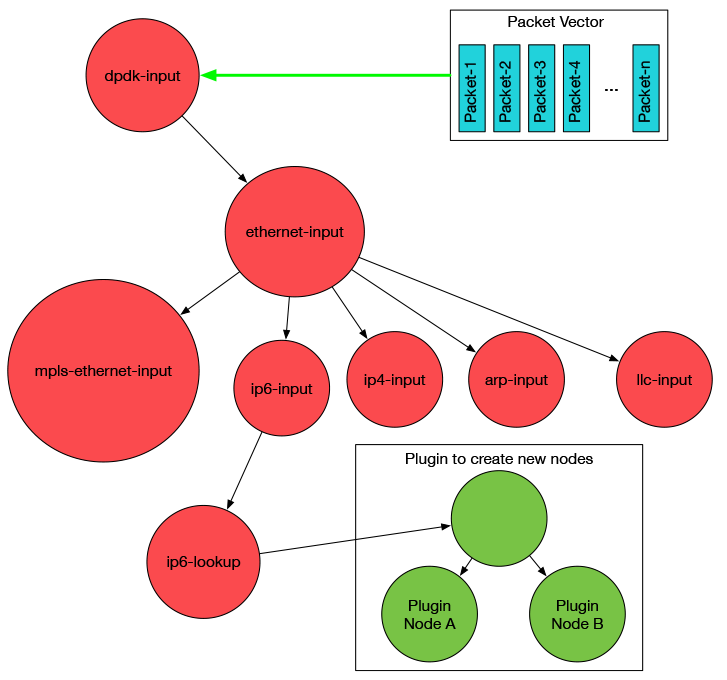
\includegraphics[scale=0.4]{images/vpp_graph.jpg}
\centering
\caption{\textit{OVS e OVS with DPDK}}
\vspace{1cm}
\label{fig:vpp_graph}
\end{figure}
\FloatBarrier

\addcontentsline{toc}{subsection}{VPP con plugin DPDK}
\subsection*{VPP con plugin DPDK}
Come si nota in \textbf{{Figura \ref{fig:vpp_graph}}}, è presente un elemento denominato \textit{dpdk-input}. Questo componente è un plugin caricato a runtime da VPP. Per abilitare il supporto a DPDK è inoltre necessario eseguire un ``binding" tra la scheda di rete e i driver DPDK. Andando a modificare il file di configurazione di VPP, un esempio chiaro di supporto ai driver DPDK può essere il seguente
\begin{minted}
[
frame=lines,
framesep=2mm,
baselinestretch=1.2,
bgcolor=white,
fontsize=\footnotesize,
highlightlines={22},
linenos
]{bash}


unix {
    nodaemon
    cli-listen /run/vpp/cli-vpp1.sock
    full-coredump
}
api-trace {
    on
    nitems 500
}
dpdk {
socket-mem 1024,2048

dev 0000:02:00.0 {
    num-rx-desc 1024
    num-rx-queues 2
}
dev 0000:01:00.0 {
    num-rx-desc 2048
    num-rx-queues 4
}
}
plugins { plugin dpdk_plugin.so {enable}}
\end{minted}
\newline
La parte evidenziata mostra come i plugin non siano altro che ``shared libraries" caricate a runtime da VPP. Il tag ``dev" indica il PCI address della scheda di rete riservata a DPDK. In questa configurazione sono presenti due schede di rete che sfruttano DPDK con due configurazioni differenti per il numero di descriptor nel buffer di ricezione e per il numero di code.